\documentclass[12pt,a4paper]{article}

% -------------------- PACKAGES --------------------
\usepackage[utf8]{inputenc}
\usepackage[T1]{fontenc}
\usepackage[english]{babel}
\usepackage{graphicx}
\usepackage{float}
\usepackage{geometry}
\geometry{top=2cm, bottom=2cm, left=2cm, right=2cm}
\usepackage{setspace}
\usepackage[table,xcdraw]{xcolor}
\usepackage{caption}
\usepackage{subcaption}
\usepackage{hyperref}
\usepackage{amsmath,amssymb}
\usepackage{booktabs}
\usepackage{listings}
\usepackage{array}
\usepackage{enumitem}

% Ruta de imagenes relativa desde informe/ hacia Workshop5/imagenes/
\graphicspath{{../imagenes/}}

% -------------------- HYPERREF SETUP --------------------
\hypersetup{
    hidelinks,
    colorlinks=true,
    breaklinks=true,
    urlcolor=blue,
    citecolor=black,
    linkcolor=black,
    pdftitle={Technical Report Workshop 5 - Coordination}
}

\setstretch{1.15}
\setlength{\parindent}{0pt}
\setlength{\parskip}{0.45em}

% -------------------- LISTINGS STYLE --------------------
\definecolor{codegreen}{rgb}{0,0.6,0}
\definecolor{codegray}{rgb}{0.5,0.5,0.5}
\definecolor{codepurple}{rgb}{0.58,0,0.82}
\definecolor{backcolour}{rgb}{0.96,0.96,0.96}

\lstset{
    backgroundcolor=\color{backcolour},
    basicstyle=\ttfamily\footnotesize,
    breaklines=true,
    frame=single,
    columns=fullflexible,
    keepspaces=true,
    showstringspaces=false,
    commentstyle=\color{codegreen},
    keywordstyle=\color{blue}\bfseries,
    stringstyle=\color{codepurple},
    numbers=left,
    numberstyle=\tiny\color{codegray},
    xleftmargin=1cm,
    xrightmargin=0.5cm
}

% -------------------- DOCUMENT --------------------
\begin{document}

% -------------------- HEADER --------------------
\noindent
\begin{minipage}{0.48\textwidth}
    \flushleft
    
\includegraphics[width=0.38\textwidth]{logo1.png}
\end{minipage}
\hfill
\begin{minipage}{0.48\textwidth}
    \flushright
    
\includegraphics[width=0.38\textwidth]{logo2.png}
\end{minipage}

\vspace{0.6cm}

\begin{center}
    {\huge \textbf{Workshop 5: Coordination}}\\[6pt]
    {\Large \textbf{Distributed Systems}}
\end{center}

\vspace{0.3cm}

\begin{center}
    \textbf{Dario Pomasqui}\\
    \textit{School of Mathematical and Computational Sciences}\\
    \textit{Yachay Tech University}\\
    Professor: Prof. Francisco Hidrobo\\
    San Miguel de Urcuqu\'{i}, Imbabura, Ecuador\\
    \textbf{GitHub Repository:} \url{https://github.com/adrianasofiaespinoza/Sistemas-Distribuidos/tree/main/Workshop5}\\
    \today
\end{center}

\vspace{0.4cm}

\begin{abstract}
This report presents the implementation and analysis of four coordination mechanisms for distributed systems: (1) centralized time synchronization via a UTC server using ZeroMQ, (2) decentralized global time synchronization inspired by the Berkeley algorithm, (3) vector clocks for causal event ordering, and (4) mutual exclusion through both a central coordinator with a FIFO queue and a distributed token ring. All implementations use Python with ZMQ for inter-process communication and threading for parallel execution. Results and discussions are provided for Parts 2, 3, and 4 as requested.
\end{abstract}

% ========================================================================
\section{Introduction}
% ========================================================================

Coordination in distributed systems involves managing the interactions and synchronization of multiple independent processes that do not share a global clock or memory. This workshop addresses four fundamental coordination problems:

\begin{itemize}
    \item \textbf{Centralized time synchronization} using a UTC server (Part 1).
    \item \textbf{Decentralized time synchronization} without a central authority (Part 2).
    \item \textbf{Causal event ordering} through vector clocks (Part 3).
    \item \textbf{Mutual exclusion} via centralized and distributed algorithms (Part 4).
\end{itemize}

All programs were implemented in Python 3 using ZeroMQ (ZMQ) for message passing and the \texttt{threading} module for concurrency. The source code is available in the GitHub repository linked above.

% ========================================================================
\section{Part 1: Coordination through UTC Server}
% ========================================================================

\subsection{Objective}

Test a client-server program where a centralized UTC server provides the current time to multiple clients. The original code was enhanced with input validation and exception handling.

\subsection{Architecture}

The system follows the ZMQ \texttt{REQ/REP} pattern. The server binds a \texttt{REP} socket on port 5000 and waits for incoming requests. Each client creates a \texttt{REQ} socket, sends a time request, and receives the UTC timestamp.

\subsection{Improvements over Original Code}

\textbf{Bug fix in client threading.} The original client code called the function immediately instead of passing it as a reference:

\begin{lstlisting}[language=Python, caption={Original (buggy)}]
# The parentheses cause immediate execution in the main thread
c.append(threading.Thread(target=utc_time_client(), args=()))
\end{lstlisting}

\begin{lstlisting}[language=Python, caption={Fixed version}]
# Pass the function reference without parentheses
t = threading.Thread(target=utc_time_client, args=())
\end{lstlisting}

\textbf{Timeout and exception handling.} The improved client sets a receive timeout to avoid blocking indefinitely if the server is unreachable:

\begin{lstlisting}[language=Python, caption={Timeout configuration}]
socket.setsockopt(zmq.RCVTIMEO, 5000)  # 5-second timeout
socket.setsockopt(zmq.LINGER, 0)       # Don't block on close
\end{lstlisting}

\textbf{Graceful server shutdown.} The server uses \texttt{socket.poll()} with a timeout instead of a blocking \texttt{recv()}, allowing it to respond to \texttt{Ctrl+C}:

\begin{lstlisting}[language=Python, caption={Non-blocking server loop}]
try:
    while True:
        if socket.poll(timeout=1000):
            message = socket.recv()
            utc_time = time.strftime('%Y-%m-%d %H:%M:%S', time.gmtime())
            socket.send_string(utc_time)
except KeyboardInterrupt:
    print("Servidor detenido")
finally:
    socket.close()
    context.term()
\end{lstlisting}

\subsection{Discussion}

The REQ/REP pattern enforces a strict request-reply sequence, making it suitable for time queries. However, this centralized approach introduces a single point of failure: if the UTC server crashes, no client can synchronize. Part 2 addresses this limitation with a decentralized approach.

% ========================================================================
\section{Part 2: Global Time without a UTC Server}
% ========================================================================

\subsection{Objective}

Simulate decentralized time synchronization where each peer node maintains its own clock, exchanges timestamps with other peers, and adjusts its local time based on the average. Random drift is introduced every $k$ cycles to model real-world clock skew.

\subsection{Algorithm}

The approach is inspired by the \textbf{Berkeley algorithm}. Each peer maintains a simulated clock:
\[T_{local} = T_{system} + \text{offset}\]

During each synchronization round:
\begin{enumerate}
    \item A peer collects timestamps from all other peers via ZMQ \texttt{REQ/REP}.
    \item It computes the average: $T_{avg} = \frac{1}{n} \sum_{i=1}^{n} T_i$
    \item It adjusts its offset: $\text{offset}_{new} = T_{avg} - T_{system}$
    \item Every $k = 2$ rounds, random drift $\in [-5, +5]$s is added.
\end{enumerate}

\subsection{Key Implementation Details}

Each peer runs a \textbf{server thread} that responds to time requests, and a \textbf{main loop} that periodically synchronizes:

\begin{lstlisting}[language=Python, caption={Clock adjustment after collecting peer times}]
if len(times) > 1:
    promedio = sum(times) / len(times)
    with self.lock:
        old = self.clock_offset
        self.clock_offset = promedio - time.time()
\end{lstlisting}

The drift injection simulates real clock inaccuracy:

\begin{lstlisting}[language=Python, caption={Periodic drift injection}]
if (r + 1) % DRIFT_EVERY_K == 0:
    drift = random.uniform(-MAX_DRIFT, MAX_DRIFT)
    with self.lock:
        self.clock_offset += drift
\end{lstlisting}

\subsection{Configuration}

\begin{table}[H]
\centering
\begin{tabular}{l l l}
\toprule
\textbf{Parameter} & \textbf{Value} & \textbf{Description} \\
\midrule
\texttt{NUM\_PEERS} & 3 & Number of peer nodes \\
\texttt{BASE\_PORT} & 6000 & Base port (6000, 6001, 6002) \\
\texttt{SYNC\_INTERVAL} & 3s & Time between rounds \\
\texttt{DRIFT\_EVERY\_K} & 2 & Add drift every 2 cycles \\
\texttt{MAX\_DRIFT} & 5s & Maximum random drift \\
\texttt{NUM\_ROUNDS} & 10 & Total synchronization rounds \\
\bottomrule
\end{tabular}
\caption{Peer node configuration}
\end{table}

\subsection{Results and Discussion}

Each peer starts with a random offset in $[-3, +3]$s. After each synchronization round, the offsets converge as each peer adjusts toward the group average. However, every 2 rounds, the injected drift disrupts convergence, and the system must re-synchronize.

The algorithm is resilient because it does not depend on a single authority. If one peer is unreachable, its time is excluded from the average, and the remaining peers still converge. The main limitation is that the average can be biased if an outlier peer reports a significantly skewed time.

\begin{figure}[H]
    \centering
    \begin{subfigure}[b]{0.48\textwidth}
        \centering
        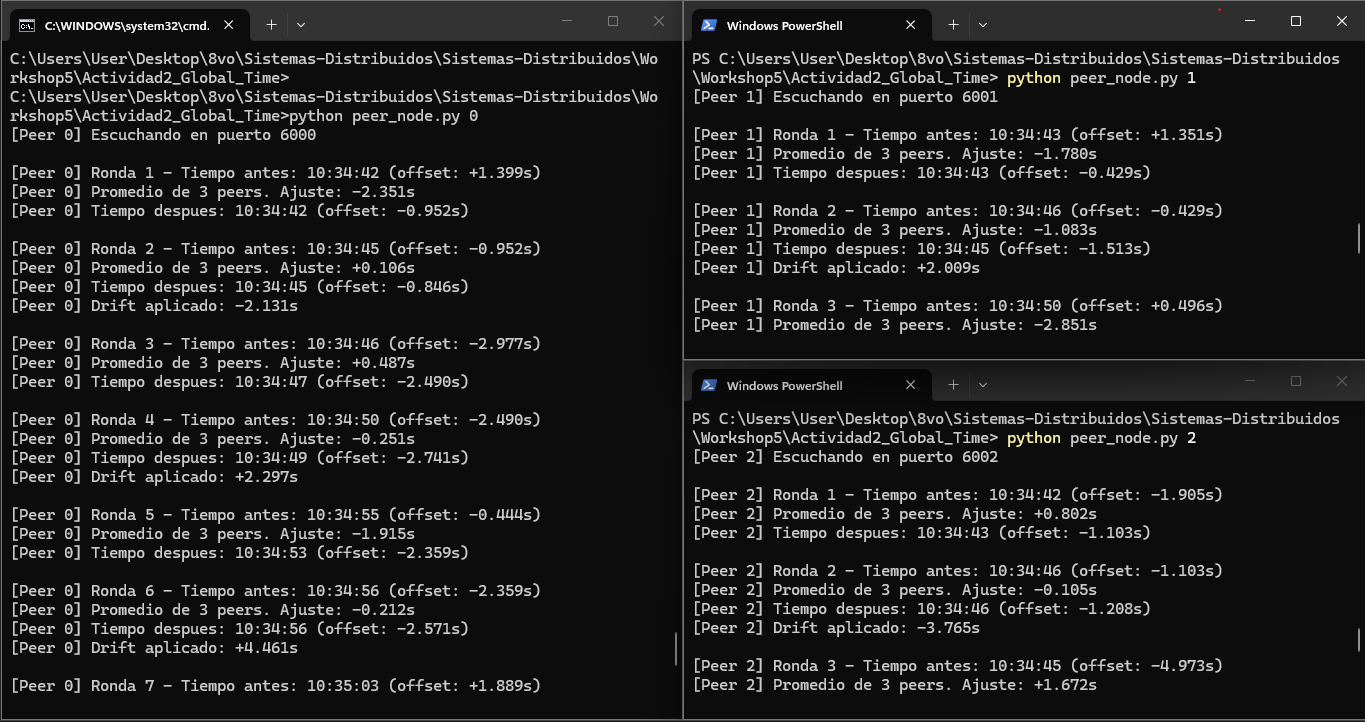
\includegraphics[width=\textwidth]{salida2final.png}
        \caption{Execution output (Part 1)}
    \end{subfigure}
    \hfill
    \begin{subfigure}[b]{0.48\textwidth}
        \centering
        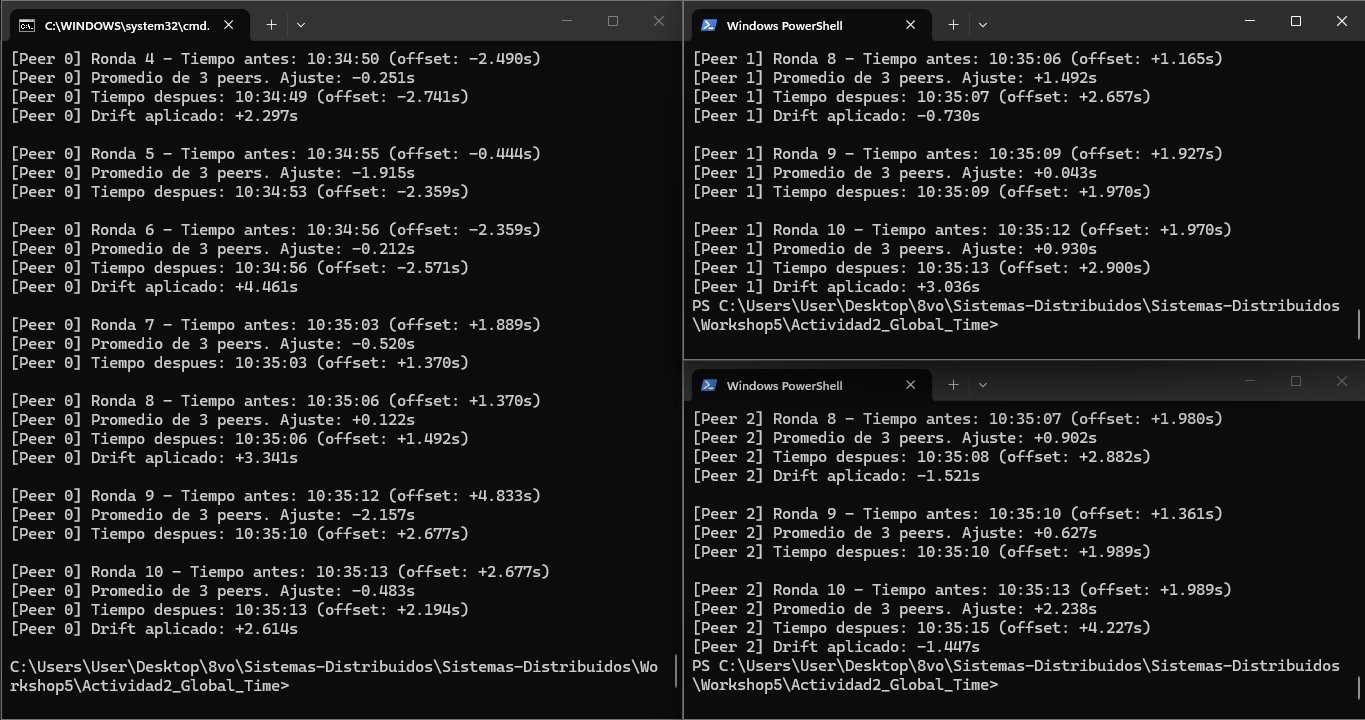
\includegraphics[width=\textwidth]{salida2final_parte2.png}
        \caption{Execution output (Part 2)}
    \end{subfigure}
    \caption{Output logs of the decentralized global time synchronization.}
\end{figure}
% ========================================================================
\section{Part 3: Vector Clocks}
% ========================================================================

\subsection{Objective}

Implement vector clocks to track causal relationships between events in a distributed system, enabling the distinction between causally ordered and concurrent events.

\subsection{Vector Clock Rules}

Given $n$ processes, each process $P_i$ maintains a vector $VC_i[0..n-1]$:

\begin{itemize}
    \item \textbf{Internal event:} $VC_i[i] \gets VC_i[i] + 1$
    \item \textbf{Send event:} $VC_i[i] \gets VC_i[i] + 1$; attach $VC_i$ to the message.
    \item \textbf{Receive event} (from $P_j$ with timestamp $TS$):
    \[\forall k: \; VC_i[k] \gets \max(VC_i[k], TS[k]), \quad \text{then } VC_i[i] \gets VC_i[i] + 1\]
\end{itemize}

Causality: $a \rightarrow b$ iff $VC(a)[k] \leq VC(b)[k]$ for all $k$ and $VC(a) \neq VC(b)$.

\subsection{Key Implementation Details}

The \texttt{VectorClock} class encapsulates the update rules. The \texttt{on\_receive} method merges the incoming clock with the local one:

\begin{lstlisting}[language=Python, caption={Vector clock merge on receive}]
def on_receive(self, other_clock):
    with self.lock:
        for i in range(self.n):
            self.clock[i] = max(self.clock[i], other_clock[i])
        self.clock[self.pid] += 1
\end{lstlisting}

Messages are serialized as JSON and transmitted via ZMQ \texttt{PUSH/PULL} sockets. Each process binds a \texttt{PULL} socket on port $7100 + \text{pid}$ and sends through temporary \texttt{PUSH} sockets:

\begin{lstlisting}[language=Python, caption={Sending a message with piggybacked vector clock}]
clock = self.vc.on_send()
msg = json.dumps({"sender": self.pid, "clock": clock})
socket.send_string(msg)
\end{lstlisting}

Events are selected randomly at each step (biased toward \texttt{send} events to generate inter-process communication). At termination, each process prints a summary of its event log.

\subsection{Results and Discussion}

With 3 processes running 8 events each, the vector clocks correctly reflect causal dependencies. For example, if $P_0$ sends a message to $P_1$ at $VC_0 = [2, 0, 0]$, and $P_1$ receives it, $P_1$'s clock becomes $[\max(VC_1[0], 2), VC_1[1]+1, \max(VC_1[2], 0)]$, correctly encoding that $P_1$ has knowledge of $P_0$'s history up to that point.

Unlike Lamport timestamps, vector clocks can determine \textbf{concurrency}: if $VC(a) \not\leq VC(b)$ and $VC(b) \not\leq VC(a)$, events $a$ and $b$ are concurrent. The trade-off is $O(n)$ overhead per message, which is acceptable for small $n$ but becomes costly at scale.

\begin{figure}[H]
    \centering
    \begin{subfigure}[b]{0.48\textwidth}
        \centering
        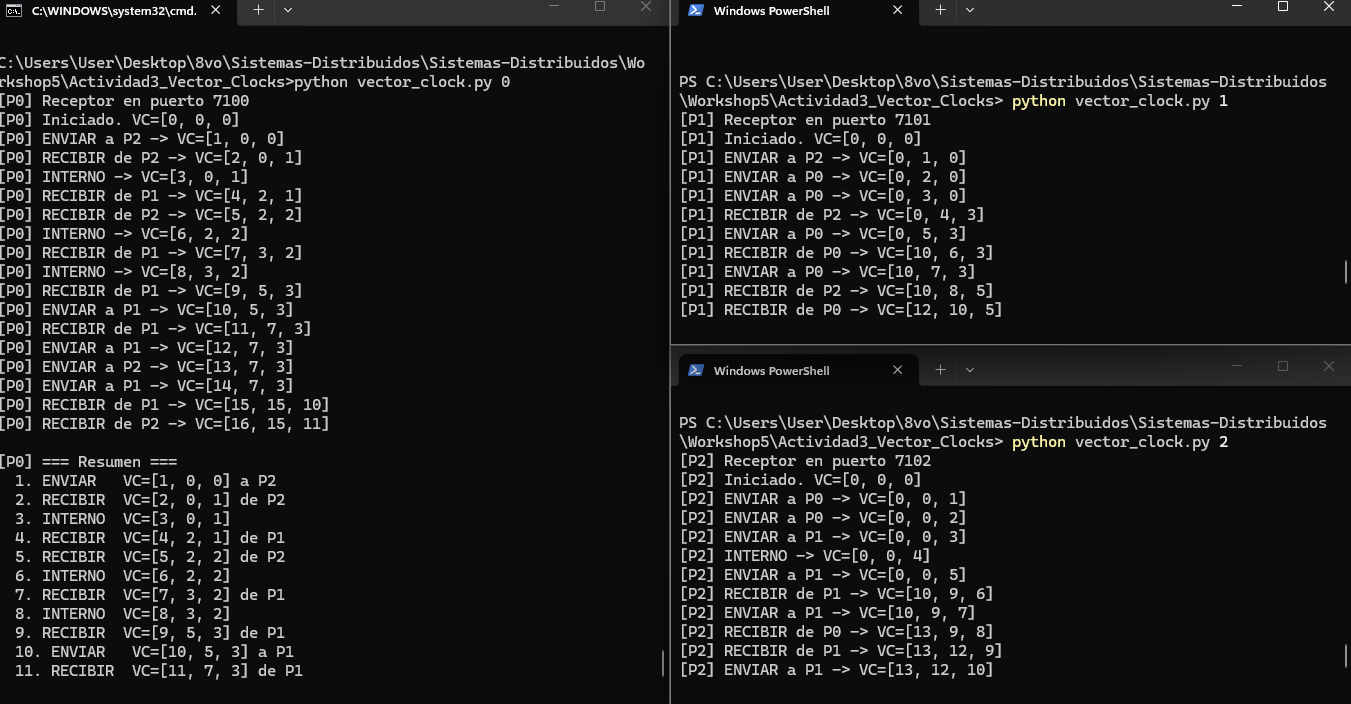
\includegraphics[width=\textwidth]{salida3_parte1.png}
        \caption{Execution output (Part 1)}
    \end{subfigure}
    \hfill
    \begin{subfigure}[b]{0.48\textwidth}
        \centering
        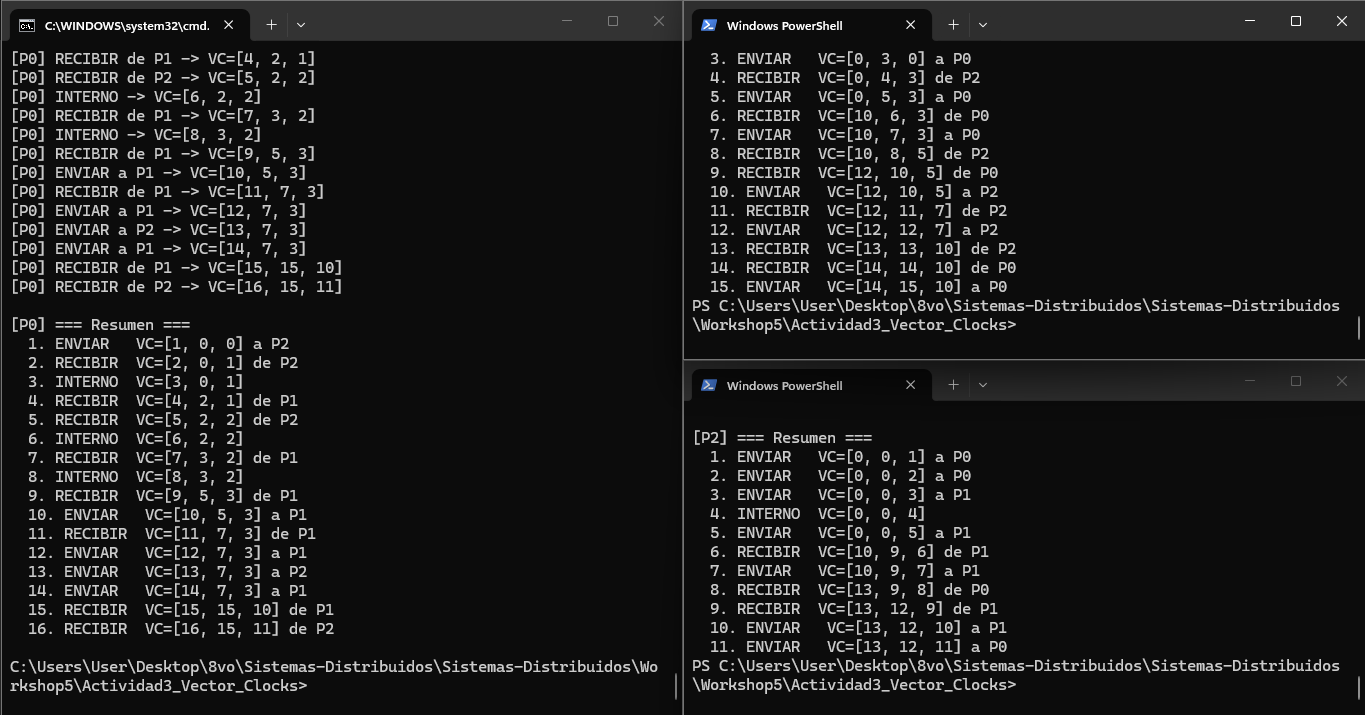
\includegraphics[width=\textwidth]{salida3_parte2.png}
        \caption{Execution output (Part 2)}
    \end{subfigure}
    \caption{Output logs of the Vector Clocks activity, showing causal ordering.}
\end{figure}

% ========================================================================
\section{Part 4: Mutual Exclusion}
% ========================================================================

\subsection{Objective}

Implement mutual exclusion guaranteeing that at most one process accesses a shared resource at any time, using two approaches: a centralized coordinator and a distributed token ring.

% -----------------------------------------------------------------------
\subsection{Approach 1: Central Resource Management Server}
% -----------------------------------------------------------------------

\subsubsection{Protocol}

The coordinator uses a ZMQ \texttt{ROUTER} socket; clients use \texttt{DEALER} sockets with unique identity strings. The message exchange follows this sequence:

\begin{enumerate}
    \item Client $\rightarrow$ Coordinator: \texttt{LOCK\_REQUEST}
    \item Coordinator $\rightarrow$ Client: \texttt{LOCK\_GRANTED} (if free) or \texttt{LOCK\_QUEUED} (if busy)
    \item Client performs work in the critical section.
    \item Client $\rightarrow$ Coordinator: \texttt{RELEASE}
    \item Coordinator grants access to next client in FIFO queue (if any).
\end{enumerate}

\subsubsection{Key Implementation Details}

The coordinator maintains a \texttt{deque} as a FIFO queue and tracks the current holder:

\begin{lstlisting}[language=Python, caption={Coordinator lock management}]
if msg == "LOCK_REQUEST":
    if self.holder is None:
        self.holder = client_id
        socket.send_multipart([client_id, b"", b"LOCK_GRANTED"])
    else:
        self.queue.append(client_id)
        socket.send_multipart([client_id, b"", b"LOCK_QUEUED"])
\end{lstlisting}

Upon release, the coordinator dequeues the next waiting client:

\begin{lstlisting}[language=Python, caption={Coordinator release handling}]
elif msg == "RELEASE":
    socket.send_multipart([client_id, b"", b"RELEASE_ACK"])
    if client_id == self.holder:
        self.holder = None
        if self.queue:
            nxt = self.queue.popleft()
            self.holder = nxt
            socket.send_multipart([nxt, b"", b"LOCK_GRANTED"])
\end{lstlisting}

% -----------------------------------------------------------------------
\subsection{Approach 2: Distributed Token Ring}
% -----------------------------------------------------------------------

\subsubsection{Protocol}

Processes form a logical ring $P_0 \to P_1 \to P_2 \to P_0$. A single token circulates; only the token holder may enter the critical section. Each process uses a \texttt{PULL} socket to receive the token and a \texttt{PUSH} socket to forward it.

\subsubsection{Key Implementation Details}

Process 0 injects the initial token into the ring:

\begin{lstlisting}[language=Python, caption={Token creation by Process 0}]
if self.pid == 0:
    time.sleep(2)
    tmp = self.context.socket(zmq.PUSH)
    tmp.setsockopt(zmq.LINGER, 1000)
    tmp.connect(f"tcp://{HOSTNAME}:{self.my_port}")
    time.sleep(0.5)
    tmp.send_string("TOKEN")
    tmp.close()
\end{lstlisting}

When the token arrives, the process decides probabilistically whether to enter the critical section:

\begin{lstlisting}[language=Python, caption={Token handling and critical section}]
token = pull.recv_string()
if token == "TOKEN":
    quiere_cs = random.random() < CS_PROB
    if quiere_cs and self.cs_count < NUM_ROUNDS:
        self.cs_count += 1
        time.sleep(random.uniform(0.5, CS_TIME))
    push.send_string("TOKEN")  # Forward token
\end{lstlisting}

\subsection{Comparison}

\begin{table}[H]
\centering
\begin{tabular}{l c c}
\toprule
\textbf{Criterion} & \textbf{Central Server} & \textbf{Token Ring} \\
\midrule
Coordination & Centralized & Distributed \\
Single point of failure & Yes & No \\
Fairness & FIFO guaranteed & Ring order \\
Messages per CS entry & 3 & $O(n)$ worst case \\
Latency (if free) & Low & Variable \\
Token loss risk & N/A & Yes (deadlock) \\
\bottomrule
\end{tabular}
\caption{Comparison of mutual exclusion approaches}
\end{table}

\subsection{Results and Discussion}

The \textbf{central server} guarantees strict FIFO fairness: the first requester is the first served. The ZMQ ROUTER/DEALER pattern allows the coordinator to identify clients by their socket identity, enabling targeted responses. The drawback is the single point of failure.

The \textbf{token ring} distributes coordination across all processes, eliminating the single point of failure. However, it introduces two issues: (1) wasted bandwidth when the token circulates among processes that do not need the resource, and (2) risk of deadlock if the token is lost (e.g., a process crashes while holding it). The probabilistic model (\texttt{CS\_PROB = 0.6}) simulates realistic workloads where not every process requires the resource each time.

Both approaches guarantee \textbf{safety} (at most one process in the critical section) and \textbf{liveness} (every request is eventually granted, assuming no failures).

\begin{figure}[H]
    \centering
    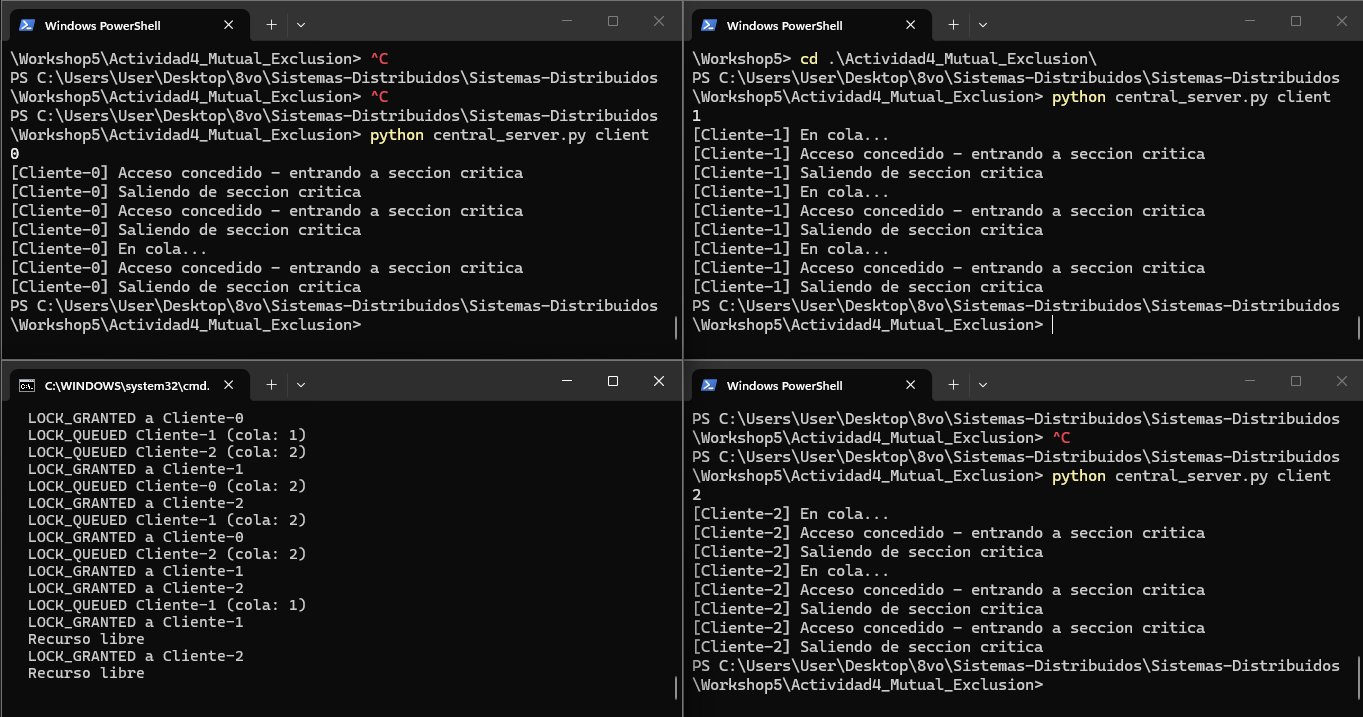
\includegraphics[width=0.7\textwidth]{Salida4.png}
    \caption{Execution output demonstrating mutual exclusion (central server and token ring).}
\end{figure}

% ========================================================================
\section{Conclusions}
% ========================================================================

\begin{itemize}
    \item \textbf{Part 1:} The centralized UTC server is simple and effective for time synchronization. Adding timeouts and exception handling improves robustness against network issues.

    \item \textbf{Part 2:} Decentralized synchronization through averaging converges toward a global time, but periodic drift disrupts convergence. The algorithm shows that coordination without a central authority is feasible but requires more rounds to stabilize.

    \item \textbf{Part 3:} Vector clocks capture causal ordering without synchronized physical clocks. They can distinguish between causally related and concurrent events, unlike Lamport timestamps, at the cost of $O(n)$ overhead per message.

    \item \textbf{Part 4:} Both mutual exclusion approaches guarantee safety. The central server provides FIFO fairness but has a single point of failure; the token ring is more fault-tolerant but introduces latency and the risk of token loss.
\end{itemize}

ZeroMQ proved versatile for all four mechanisms, offering appropriate socket patterns for each communication need: REQ/REP for request-reply, PUSH/PULL for unidirectional messaging, and ROUTER/DEALER for multiplexed client-server interaction.

% ========================================================================
\section{References}
% ========================================================================

\begin{enumerate}
    \item Coulouris, G., Dollimore, J., Kindberg, T., \& Blair, G. (2012). \textit{Distributed Systems: Concepts and Design}. 5th Edition. Addison-Wesley.
    \item Tanenbaum, A. S., \& Van Steen, M. (2017). \textit{Distributed Systems: Principles and Paradigms}. 3rd Edition. Pearson.
    \item ZeroMQ Documentation. \url{https://zeromq.org/}
    \item Lamport, L. (1978). Time, Clocks, and the Ordering of Events in a Distributed System. \textit{Communications of the ACM}, 21(7), 558--565.
    \item Fidge, C. J. (1988). Timestamps in Message-Passing Systems That Preserve the Partial Ordering. \textit{Proceedings of the 11th Australian Computer Science Conference}.
\end{enumerate}

\end{document}
